\chapter{Planen}\label{ch:planen}
In diesem Abschnitt, wird die Planung beschrieben. In dieser Phase werden basierend auf den Anforderungen Arbeitspakete erstellt, und in einem GANT-Diagramm auf die 10 Tage eingeteilt.

\section{Arbeitspakete}

Um den ganzen Auftrag in kleine übersichtliche Teile aufzuteilen, wird er in verschiedene kleine Arbeitspakete unterteilt. Die Arbeitspakete sind jeweils nummeriert, haben einen Namen, einen geschätzten Aufwand in h und eine \flqq Definition of Done\frqq{}/ ein erwartetes Ergebnis. Die Aufwände sind oft mit einem gewissen Puffer geschätzt.\\
Die Pakete  sind nach den 6 Phasen der IPERKA Methode aufgelistet. Arbeiten welche IPA-spezifisch sind, sind unter Rahmenaufgaben aufgeführt.

\subsection{Informieren}
Hier, sind die Arbeitspakete, welche während der IPERKA-Phase \flqq Informieren\frqq{}\space bearbeitet wurden, aufgelistet.

\begin{longtable}{p{.22\textwidth}|p{.78\textwidth}}
	\hline
	\textbf{Nummer}    				& 1.1 \\
	\hline
	\textbf{Name}   				& Projektumfeld analysieren und beschreiben \\
	\hline
	\textbf{Geschätzter Aufwand}	& 2h \\
	\hline
	\textbf{Erwartetes Ergebnis}	& Das Ziel der Arbeit ist klar, ein grober Überblick besteht. \\
	\hline
\end{longtable}

\begin{longtable}{p{.22\textwidth}|p{.78\textwidth}}
	\hline
	\textbf{Nummer}    				& 1.2 \\
	\hline
	\textbf{Name}   				& Anforderungen definieren \\
	\hline
	\textbf{Geschätzter Aufwand}	& 2h \\
	\hline
	\textbf{Erwartetes Ergebnis}	& Die funktionalen und nicht-funktionalen Anforderungen sind definiert und beschrieben\\
	\hline
\end{longtable}\pagebreak

\subsection{Planen}
Hier, sind die Arbeitspakete, welche während der IPERKA-Phase \flqq Planen\frqq{}\space bearbeitet werden, aufgelistet.

\begin{longtable}{p{.22\textwidth}|p{.78\textwidth}}
	\hline
	\textbf{Nummer}    				& 2.1 \\
	\hline
	\textbf{Name}   				& Arbeitspakete definieren \\
	\hline
	\textbf{Geschätzter Aufwand}	& 3h \\
	\hline
	\textbf{Erwartetes Ergebnis}	& Die ganze Arbeit ist in kleine logische Arbeitspakete unterteilt. Alle Arbeitspakete sind klar definiert.\\
	\hline
\end{longtable}

\begin{longtable}{p{.22\textwidth}|p{.78\textwidth}}
	\hline
	\textbf{Nummer}    				& 2.2 \\
	\hline
	\textbf{Name}   				& Zeitplan erstellen \\
	\hline
	\textbf{Geschätzter Aufwand}	& 1h \\
	\hline
	\textbf{Erwartetes Ergebnis}	& Der GANT-Zeitplan ist anhand der Arbeitspakete erstellt. Es sind alle Arbeitspakete vorhanden.\\
	\hline
\end{longtable}

\begin{longtable}{p{.22\textwidth}|p{.78\textwidth}}
	\hline
	\textbf{Nummer}    				& 2.3 \\
	\hline
	\textbf{Name}   				& Lösungskonzept für das Backend erarbeiten\\
	\hline
	\textbf{Geschätzter Aufwand}	& 4h \\
	\hline
	\textbf{Erwartetes Ergebnis}	& Es ist mindestens ein Lösungsvorschlag definiert und so weit wie Sinnvoll beschrieben und durchgedacht. Der relevante Backendcode ist verstanden.\\
	\hline
\end{longtable}\pagebreak

\begin{longtable}{p{.22\textwidth}|p{.78\textwidth}}
	\hline
	\textbf{Nummer}    				& 2.4 \\
	\hline
	\textbf{Name}   				& Lösungskonzept für die SPA erarbeiten\\
	\hline
	\textbf{Geschätzter Aufwand}	& 4h \\
	\hline
	\textbf{Erwartetes Ergebnis}	& Es ist mindestens ein Lösungsvorschlag definiert und so weit wie Sinnvoll beschrieben und durchgedacht. Es sind verschiedene Mockups vorhanden, und der relevante SPA Code ist verstanden.\\
	\hline
\end{longtable}

\begin{longtable}{p{.22\textwidth}|p{.78\textwidth}}
	\hline
	\textbf{Nummer}    				& 2.5 \\
	\hline
	\textbf{Name}   				& Test- und Qualitätssicherungskonzept erstellen\\
	\hline
	\textbf{Geschätzter Aufwand}	& 4h \\
	\hline
	\textbf{Erwartetes Ergebnis}	& Das Testkonzept ist erstellt und dokumentiert. Das Qualitätssicherungskonzept ist erstellt und dokumentiert.\\
	\hline
\end{longtable}

\subsection{Entscheiden}
Hier, sind die Arbeitspakete, welche während der IPERKA-Phase \flqq Entscheiden\frqq{}\space bearbeitet werden, aufgelistet.

\begin{longtable}{p{.22\textwidth}|p{.78\textwidth}}
	\hline
	\textbf{Nummer}    				& 3.1 \\
	\hline
	\textbf{Name}   				& Lösungsvarianten evaluieren \\
	\hline
	\textbf{Geschätzter Aufwand}	& 2h \\
	\hline
	\textbf{Erwartetes Ergebnis}	& Aus den verschiedenen Lösungsvarianten der SPA und des Backends wurde sich für eine entschieden, und dies Dokumentiert.\\
	\hline
\end{longtable}\pagebreak

\subsection{Realisieren}
Hier, sind die Arbeitspakete, welche während der IPERKA-Phase \flqq Realisieren\frqq{}\space bearbeitet werden, aufgelistet.

\begin{longtable}{p{.22\textwidth}|p{.78\textwidth}}
	\hline
	\textbf{Nummer}    				& 4.1 \\
	\hline
	\textbf{Name}   				& Das Backend erweitern  \\
	\hline
	\textbf{Geschätzter Aufwand}	& 14h \\
	\hline
	\textbf{Erwartetes Ergebnis}	& Alle Anforderungen für das Backend sind nach dem definierten Lösungsansatz umgesetzt. Zugleich ist die Lösung dokumentiert \\
	\hline
\end{longtable}

\begin{longtable}{p{.22\textwidth}|p{.78\textwidth}}
	\hline
	\textbf{Nummer}    				& 4.2 \\
	\hline
	\textbf{Name}   				& Unit- und Integrationtests schreiben  \\
	\hline
	\textbf{Geschätzter Aufwand}	& 6h \\
	\hline
	\textbf{Erwartetes Ergebnis}	& Alle neuen Funktionalitäten sind mit Unit- und/oder Integrationtests getestet.\\
	\hline
\end{longtable}


\begin{longtable}{p{.22\textwidth}|p{.78\textwidth}}
	\hline
	\textbf{Nummer}    				& 4.3 \\
	\hline
	\textbf{Name}   				& Die SPA erweitern  \\
	\hline
	\textbf{Geschätzter Aufwand}	& 6h \\
	\hline
	\textbf{Erwartetes Ergebnis}	& Alle Anforderungen für die SPA sind nach dem definierten Lösungsansatz umgesetzt. Zugleich ist die Lösung dokumentiert.\\
	\hline
\end{longtable}

\begin{longtable}{p{.22\textwidth}|p{.78\textwidth}}
	\hline
	\textbf{Nummer}    				& 4.4 \\
	\hline
	\textbf{Name}   				& Selenium Integrationtests implementieren  \\
	\hline
	\textbf{Geschätzter Aufwand}	& 5h \\
	\hline
	\textbf{Erwartetes Ergebnis}	& Alle neuen Funktionalitäten sind mit Selenium Integrationtests getestet.\\
	\hline
\end{longtable}\pagebreak

\begin{longtable}{p{.22\textwidth}|p{.78\textwidth}}
	\hline
	\textbf{Nummer}    				& 4.5 \\
	\hline
	\textbf{Name}   				& Kundendokumentation schreiben  \\
	\hline
	\textbf{Geschätzter Aufwand}	& 2h \\
	\hline
	\textbf{Erwartetes Ergebnis}	& Die neue Funktionalität ist in der Kundendokumentation dokumentiert, und alle Anforderungen sind erfüllt.\\
	\hline
\end{longtable}


\subsection{Kontrollieren}
Hier, sind die Arbeitspakete, welche während der IPERKA-Phase \flqq Kontrollieren\frqq{}\space bearbeitet werden, aufgelistet.

\begin{longtable}{p{.22\textwidth}|p{.78\textwidth}}
	\hline
	\textbf{Nummer}    				& 5.1 \\
	\hline
	\textbf{Name}   				& Tests durchführen, und Fehler beheben \\
	\hline
	\textbf{Geschätzter Aufwand}	& 4h
	h \\
	\hline
	\textbf{Erwartetes Ergebnis}	& Tests sind gemäss Testkonzept durchgeführt, und mögliche Fehler sind behoben. \\
	\hline
\end{longtable}

\begin{longtable}{p{.22\textwidth}|p{.78\textwidth}}
	\hline
	\textbf{Nummer}    				& 5.2 \\
	\hline
	\textbf{Name}   				& Codequalität prüfen, und Refactorn \\
	\hline
	\textbf{Geschätzter Aufwand}	& 1h \\
	\hline
	\textbf{Erwartetes Ergebnis}	& Code ist nochmals durchgeschaut, und Unschönheiten sind bereinigt.\\
	\hline
\end{longtable}

\begin{longtable}{p{.22\textwidth}|p{.78\textwidth}}
	\hline
	\textbf{Nummer}    				& 5.3 \\
	\hline
	\textbf{Name}   				& Dokumentation finalisieren \\
	\hline
	\textbf{Geschätzter Aufwand}	& 8h \\
	\hline
	\textbf{Erwartetes Ergebnis}	& Die Dokumentation ist soweit wie möglich finalisiert und entspricht den Vorgaben.\\
	\hline
\end{longtable}

\subsection{Auswerten}
Hier, sind die Arbeitspakete, welche während der letzten IPERKA-Phase \flqq Auswerten\frqq{}\space bearbeitet werden, aufgelistet.

\begin{longtable}{p{.22\textwidth}|p{.78\textwidth}}
	\hline
	\textbf{Nummer}    				& 6.2 \\
	\hline
	\textbf{Name}   				& Reflexion schreiben \\
	\hline
	\textbf{Geschätzter Aufwand}	& 2h \\
	\hline
	\textbf{Erwartetes Ergebnis}	& Reflexion zu den relevanten Abschnitten ist geschrieben. \\
	\hline
\end{longtable}

\subsection{Rahmenaufgaben}
Hier, sind die Arbeitspakete, welche IPA-spezifische Arbeit erfordern, aufgelistet.

\begin{longtable}{p{.22\textwidth}|p{.78\textwidth}}
	\hline
	\textbf{Nummer}    				& 7.1 \\
	\hline
	\textbf{Name}   				& Projektstruktur aufsetzen\\
	\hline
	\textbf{Geschätzter Aufwand}	& 2h \\
	\hline
	\textbf{Erwartetes Ergebnis}	& Das Grundgerüst für den Bericht steht. Der Latex-Build ist lauffähig und generiert ein anschaubares PDF.\\
	\hline
\end{longtable}

\begin{longtable}{p{.22\textwidth}|p{.78\textwidth}}
	\hline
	\textbf{Nummer}    				& 7.2 \\
	\hline
	\textbf{Name}   				& Aufgabenstellung und Rahmenbedingungen beschreiben\\
	\hline
	\textbf{Geschätzter Aufwand}	& 1h \\
	\hline
	\textbf{Erwartetes Ergebnis}	& Die Aufgabenstellung ist in den Bericht übernommen. Benützte Firmenstandarts sowie die Projektaufbauorganisation sind defniert und beschrieben. \\
	\hline
\end{longtable}

\newpage

\begin{longtable}{p{.22\textwidth}|p{.78\textwidth}}
	\hline
	\textbf{Nummer}    				& 7.3 \\
	\hline
	\textbf{Name}   				& Projektmanagementmethode definieren\\
	\hline
	\textbf{Geschätzter Aufwand}	& 1h \\
	\hline
	\textbf{Erwartetes Ergebnis}	& Es steht fest mit welcher Projektmanagementmethode die Probe-IPA umgesetzt werden soll. Der Bericht wurde so gegliedert.\\
	\hline
\end{longtable}

\begin{longtable}{p{.22\textwidth}|p{.78\textwidth}}
	\hline
	\textbf{Nummer}    				& 7.4 \\
	\hline
	\textbf{Name}   				& Expertenbesuche\\
	\hline
	\textbf{Geschätzter Aufwand}	& 4h \\
	\hline
	\textbf{Erwartetes Ergebnis}	& Infos aus dem Gespräch sind am richtigen Ort festgehalten.\\
	\hline
\end{longtable}

\begin{longtable}{p{.22\textwidth}|p{.78\textwidth}}
	\hline
	\textbf{Nummer}    				& 7.5 \\
	\hline
	\textbf{Name}   				& Anhang erstellen\\
	\hline
	\textbf{Geschätzter Aufwand}	& 2h \\
	\hline
	\textbf{Erwartetes Ergebnis}	& Der Anhang ist erstellt und beinhaltet alle nötigen und verlangten Inhalte.\\
	\hline
\end{longtable} 
\newpage

\section{Lösungskonzept Backend}

In diesem Kapitel ist das Lösungskonzept für das Backend beschrieben. Das Konzept richtet sich nach den in Kapitel \ref{subsec:anforderungenBackend} definierten Anforderungen.

\subsection{REST}

Damit die SPA den 16-stelligen Aktivierungscode anzeigen kann, muss er mit Hilfe einer REST-Schnittstelle übermittelt werden. Dass er aber überhaupt von Futurae erstellt wird, muss er bei dem Enrollement, also dem Call der einen neuen Nutzer erstellt, explizit gefordert werden. 
Dies funktioniert in dem man den Requestparameter \flqq short\_code\frqq{} auf true setzt. Für die Übermittlung an die SPA stehen 2 Optionen im Raum:

\begin{itemize}
	\item Option 1: Den Endpunkt, welcher alle Accountdaten von jedem Nutzer zurück gibt um den Activation Code erweitern. Dies hätte zur Folge das der Endpunkt um ein optionales Feld \flqq activation\_code\_short\frqq{}\space erweitert wird.
	\label{"itm:restOption1"}
	\item Option 2: Einen neuen Endpunkt erstellen, welcher den offenen Aktivierungscode zurück gibt. Dies wäre ein einfacher GET-Endpunkte, welcher, falls vorhanden den neusten, austehenden Aktivierungscode zurück gibt. Folgend eine kurze Spezifikation des Endpunktes:\\\\

	\textbf{Pfad:} /auth-admin/rest/users/{userId}/tokens/airlock-2fa/activation-code-short\\
	\textbf{HTTP-Methode:} GET\\
	\textbf{Pfadparameter:} userid\\
	\textbf{Response:} Optionaler Actiovation Code, kann leer sein \newline
	\textbf{Status Codes:}
	\begin{longtable}{p{.25\textwidth}|p{.55\textwidth}}
		\hline
		\textbf{200 Ok}    				& 16-stelliger Activationcode oder nichts \\
		\hline
		\textbf{401 Unauthorized}   				& Invalide oder fehlende Authentifizierung\\
		\hline
		\textbf{403 Forbidden}	& Der Zugriff ist verboten (z.B falsche Adminrolle) \\
		\hline
		\textbf{404 Not Found}	& Mögliche Error Codes:
		\begin{itemize}
			\item USER\_NOT\_FOUND 
			\item ACCOUNT\_NOT\_FOUND
		\end{itemize}\\
		\hline
	\end{longtable} 
	
	\label{"itm:restOption2"}	
\end{itemize}

In beiden Fällen müsste der Restflow so aussehen:
\begin{figure}[H]
	\begin{center}
		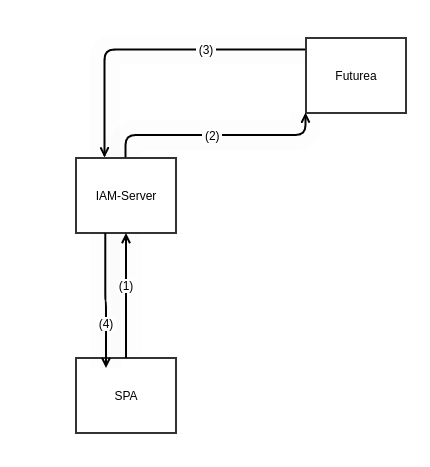
\includegraphics[width=0.8\textwidth]{ressourcen/restflow}
		\caption[Restflow]{Restflow um 16-stelligen Aktivierungscode zu bekommen}\label{fig:restflow}
	\end{center}
\end{figure}

\begin{itemize}
	\item[(1)] Die SPA macht als Reaktion auf einen Klick einen Request, ans IAM Backend. Je nach Option, geht dieser an einen anderen Endpunkt. 
	\item[(2)] Das Backend macht folgenden Request an Futurae: \newline
	/srv/admin/v1/enrollments?status=pending
	\item[(3)] 	Da bei dem Enrollment Request zu Futurea der 16-stellige Activationcode explizit gefordert wurde, wird dieser Request, falls überhaupt ein austehendes Enrollment vorhanden ist, dieses auch zurück geben. Da mehere offene Enrollments vorhanden sein können, muss immer das Neuste genommen werden. Damit immer klar ist welcher Code zurück kommt. Helpdesk oder Schalter Mitarbeiter können so die Aktivierung direkt mit dem Kunden durchspielen.
	\item[(4)] Das Backend gibt den Activationcode an die SPA weiter. Je nach Option auch noch die anderen Accountdaten. Falls keiner vorhanden ist, wird die Response einfach leer gelassen, resp. das Feld.
\end{itemize}


\subsection{Rollenlogik}
Es gibt bereits eine Regel, welche das Ansehen von Aktivierungsdaten einschränkt. Diese Regel kann wiederverwendet werden. Dazu gibt es einen Airlock2FAAccessController.java. Dieser kann beim erstellen der Response injected werden. Mit der Methode \flqq isAllowedToSeeActivationSecrets\frqq{} \space kann dann überprüft werden, ob der Adminnutzer diese Info überhaupt sehen darf. Am besten wird dieser Check noch vor dem Futurae Request ausgführt, um einen unnötigen Rountrip zu vermeiden und es möglichst effizient zu halten.


\section{Lösungskonzept SPA}
